\documentclass[10pt,t,xcolor=dvipsnames]{beamer}

\usetheme{Antibes}
\usecolortheme{structure}
%\usepackage[utf8x]{inputenc}
%\usepackage{default}
%\usecolortheme{albatross}
%\usecolortheme{lily}
%\usecolortheme{sidebartab}
%\usecolortheme{crane}
%\usecolortheme{orchid}
%\usecolortheme{albatross}
%\usecolortheme{beetle}
%\usecolortheme{dove}
%\usecolortheme{fly}
%\usecolortheme{seagull}
%\usecolortheme{dolphin}
%\usecolortheme{rose}
\usepackage{graphics}
% \usepackage[pdftex]{graphicx}
\usepackage{graphicx}
\usepackage{xcolor}
\usepackage{color}
%\usepackage{url}
\usepackage{hyperref}
%\usepackage[obeyspaces]{url}
\usepackage{amssymb,amsmath} % for the bold symbol command
\usepackage{booktabs} % toprule etc in tables
\usepackage{mathrsfs}
\usepackage{listings}
\lstset{ %
  backgroundcolor=\color{white},
  basicstyle=\footnotesize,
  breakatwhitespace=false,
  breaklines=true,
  captionpos=b,
  commentstyle=\color{green},
  escapeinside={\%*}{*)},
  extendedchars=true,
  frame=single,
  keywordstyle=\color{blue},
  language=bash,
  numbers=left,
  numbersep=5pt,
  numberstyle=\tiny\color{gray},
  rulecolor=\color{black},
  showspaces=false,
  showstringspaces=false,
  showtabs=false,
  stepnumber=2,
  stringstyle=\color{red},
  tabsize=2,
  title=\lstname,
  morekeywords={not,\},\{,preconditions,effects },
  deletekeywords={time}
}
%\usepackage{minted}
%\usepackage{beamerthemebars}
%\usepackage{ragged2e}
%\usepackage{lipsum}

\setbeamercolor{structure}{fg=MidnightBlue!50!black}
\renewcommand{\raggedright}{\leftskip=0pt \rightskip=0pt plus 0cm}
\logo{
\includegraphics[scale=0.05]{../../../TWAssets/TW_Colour_Logos_trans_green.png}}

\title{ More on Web Development Basics }
\titlegraphic{
\includegraphics[scale=0.15]{../../../TWAssets/TW_Colour_Logos_trans_green.png}}

\author{ Patrick Turley \& 'Wole Solana }
\begin{document}
\nocite*{}
\frame [c, plain]{\titlepage}
%-------------------------------Slide1-------------------------------
\begin{frame}[fragile]
\frametitle{Why use a web framework?}
\pause
\begin{columns}[l]
\column{0.5\textwidth}
\begin{figure}
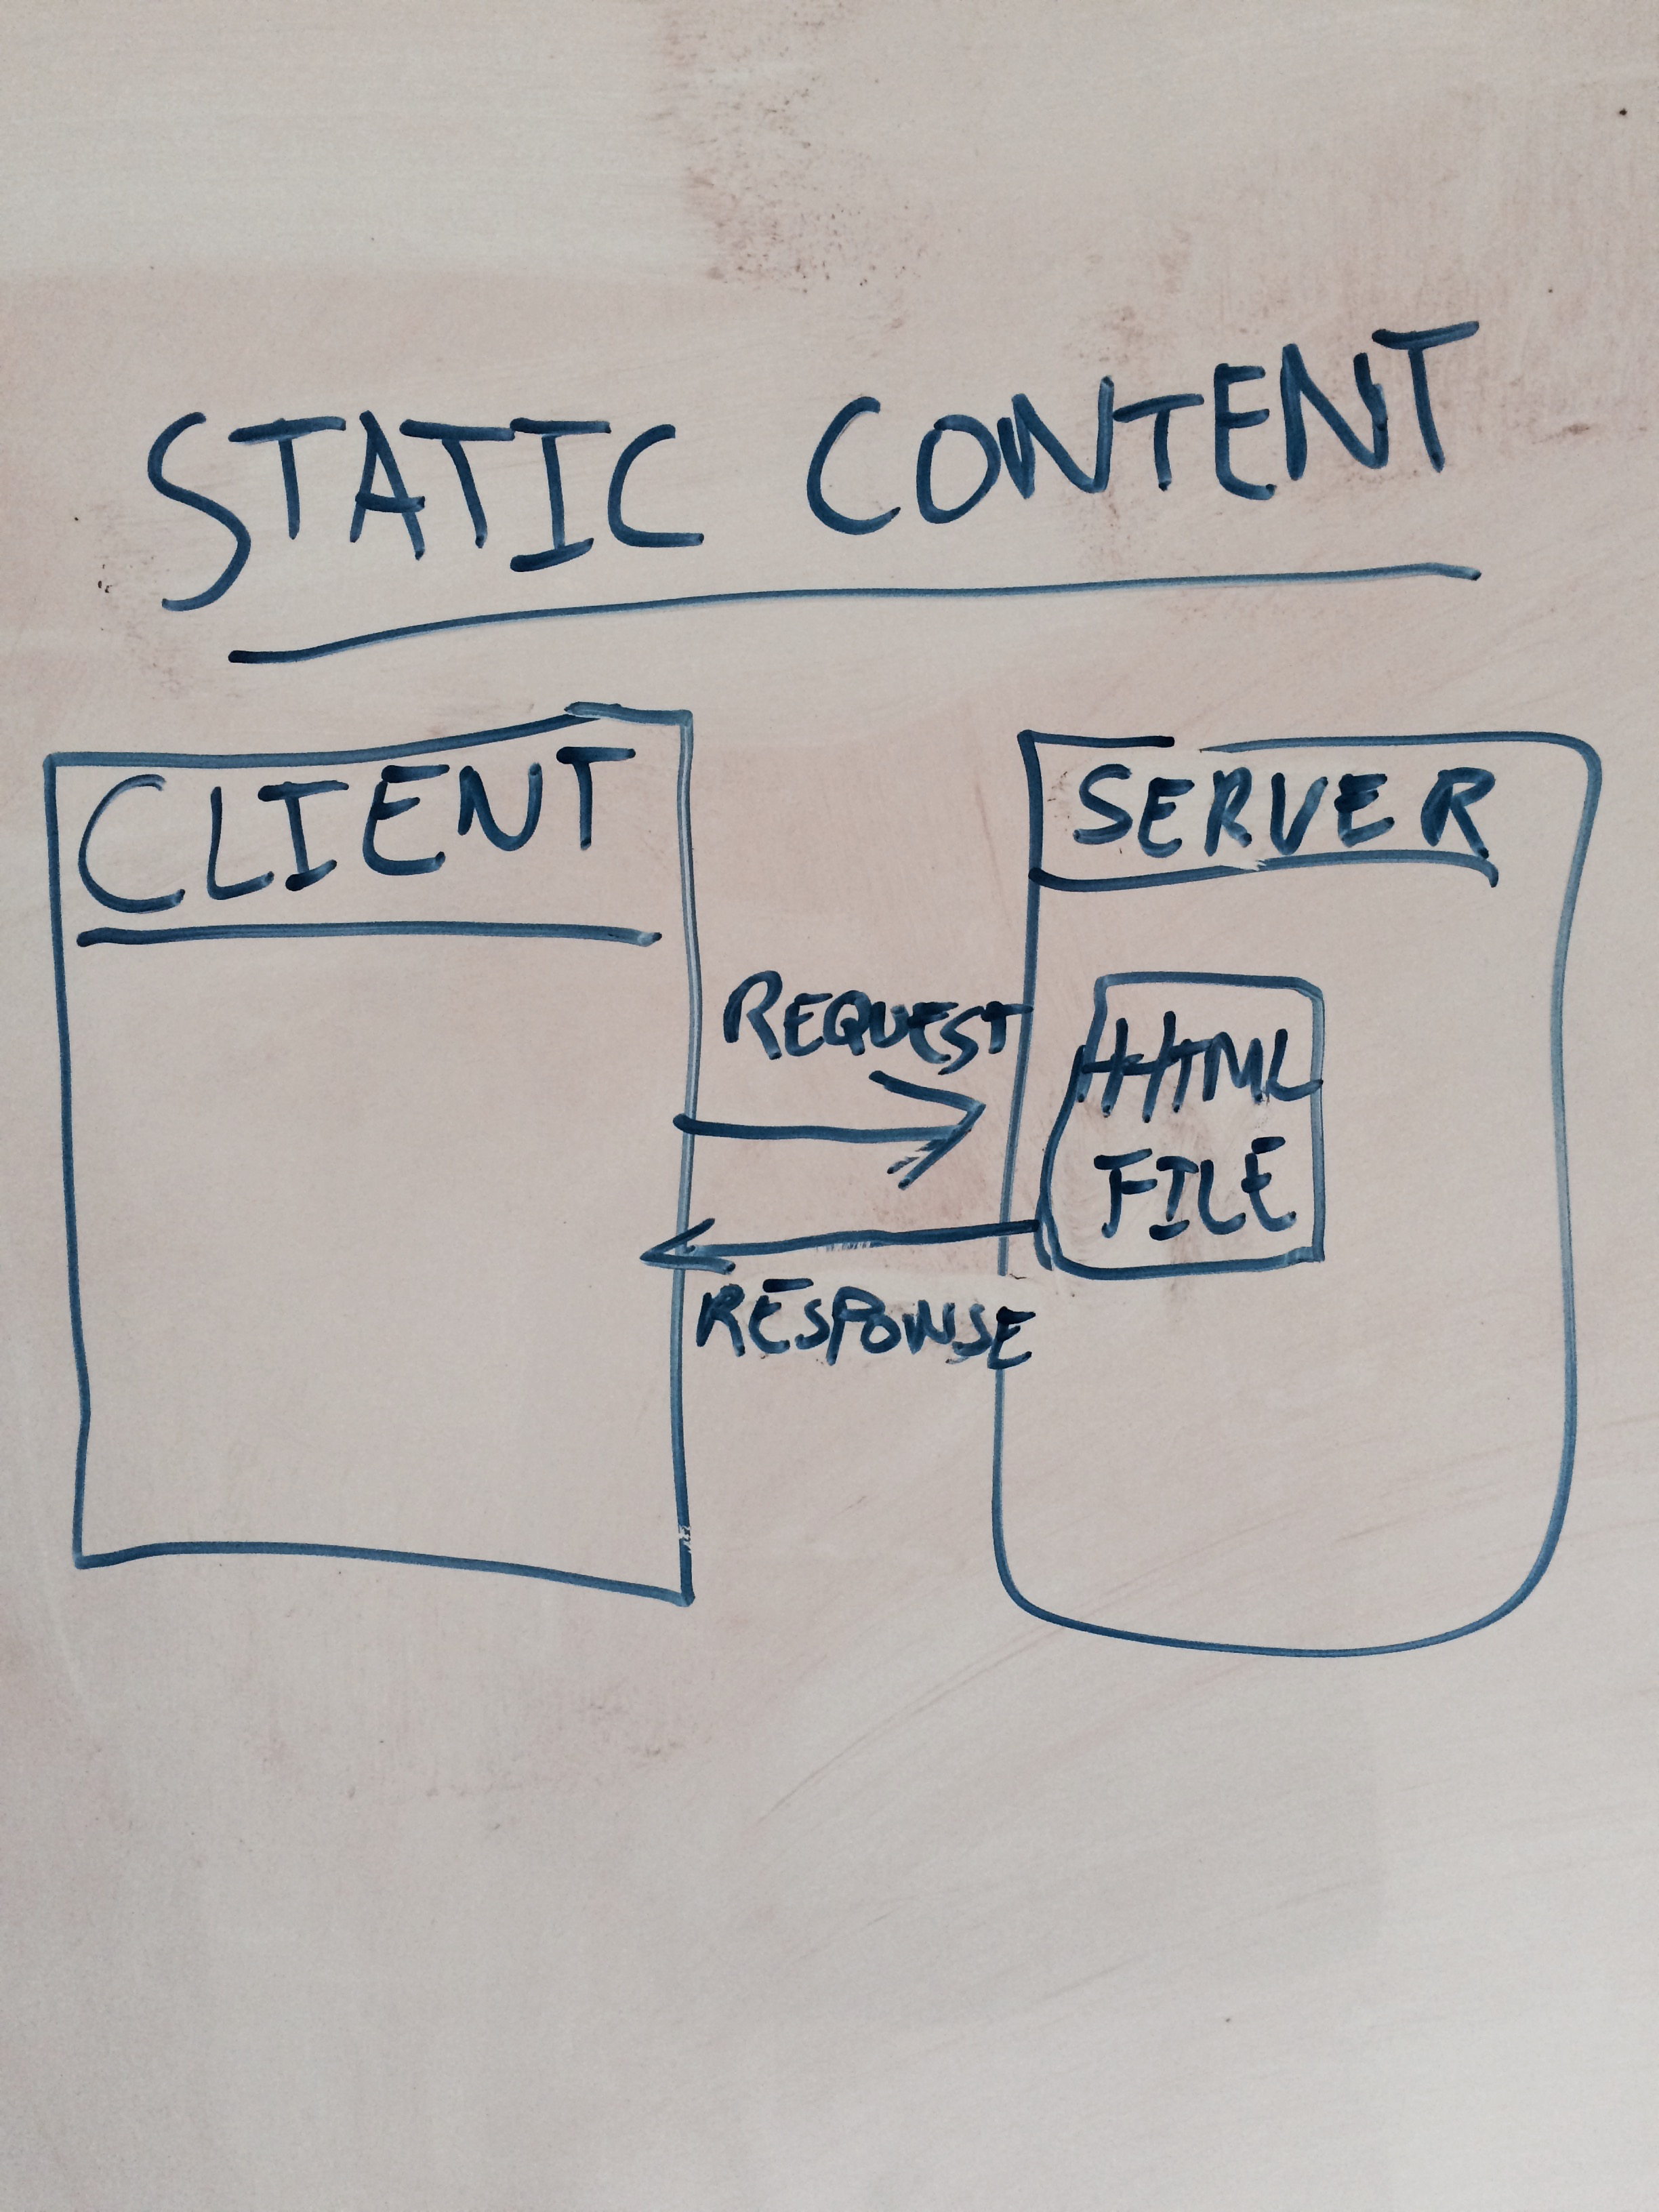
\includegraphics[scale=0.05]{../images/static.jpg}
\caption{Static Content}
\end{figure}
\pause
\column{0.5\textwidth}
\begin{figure}
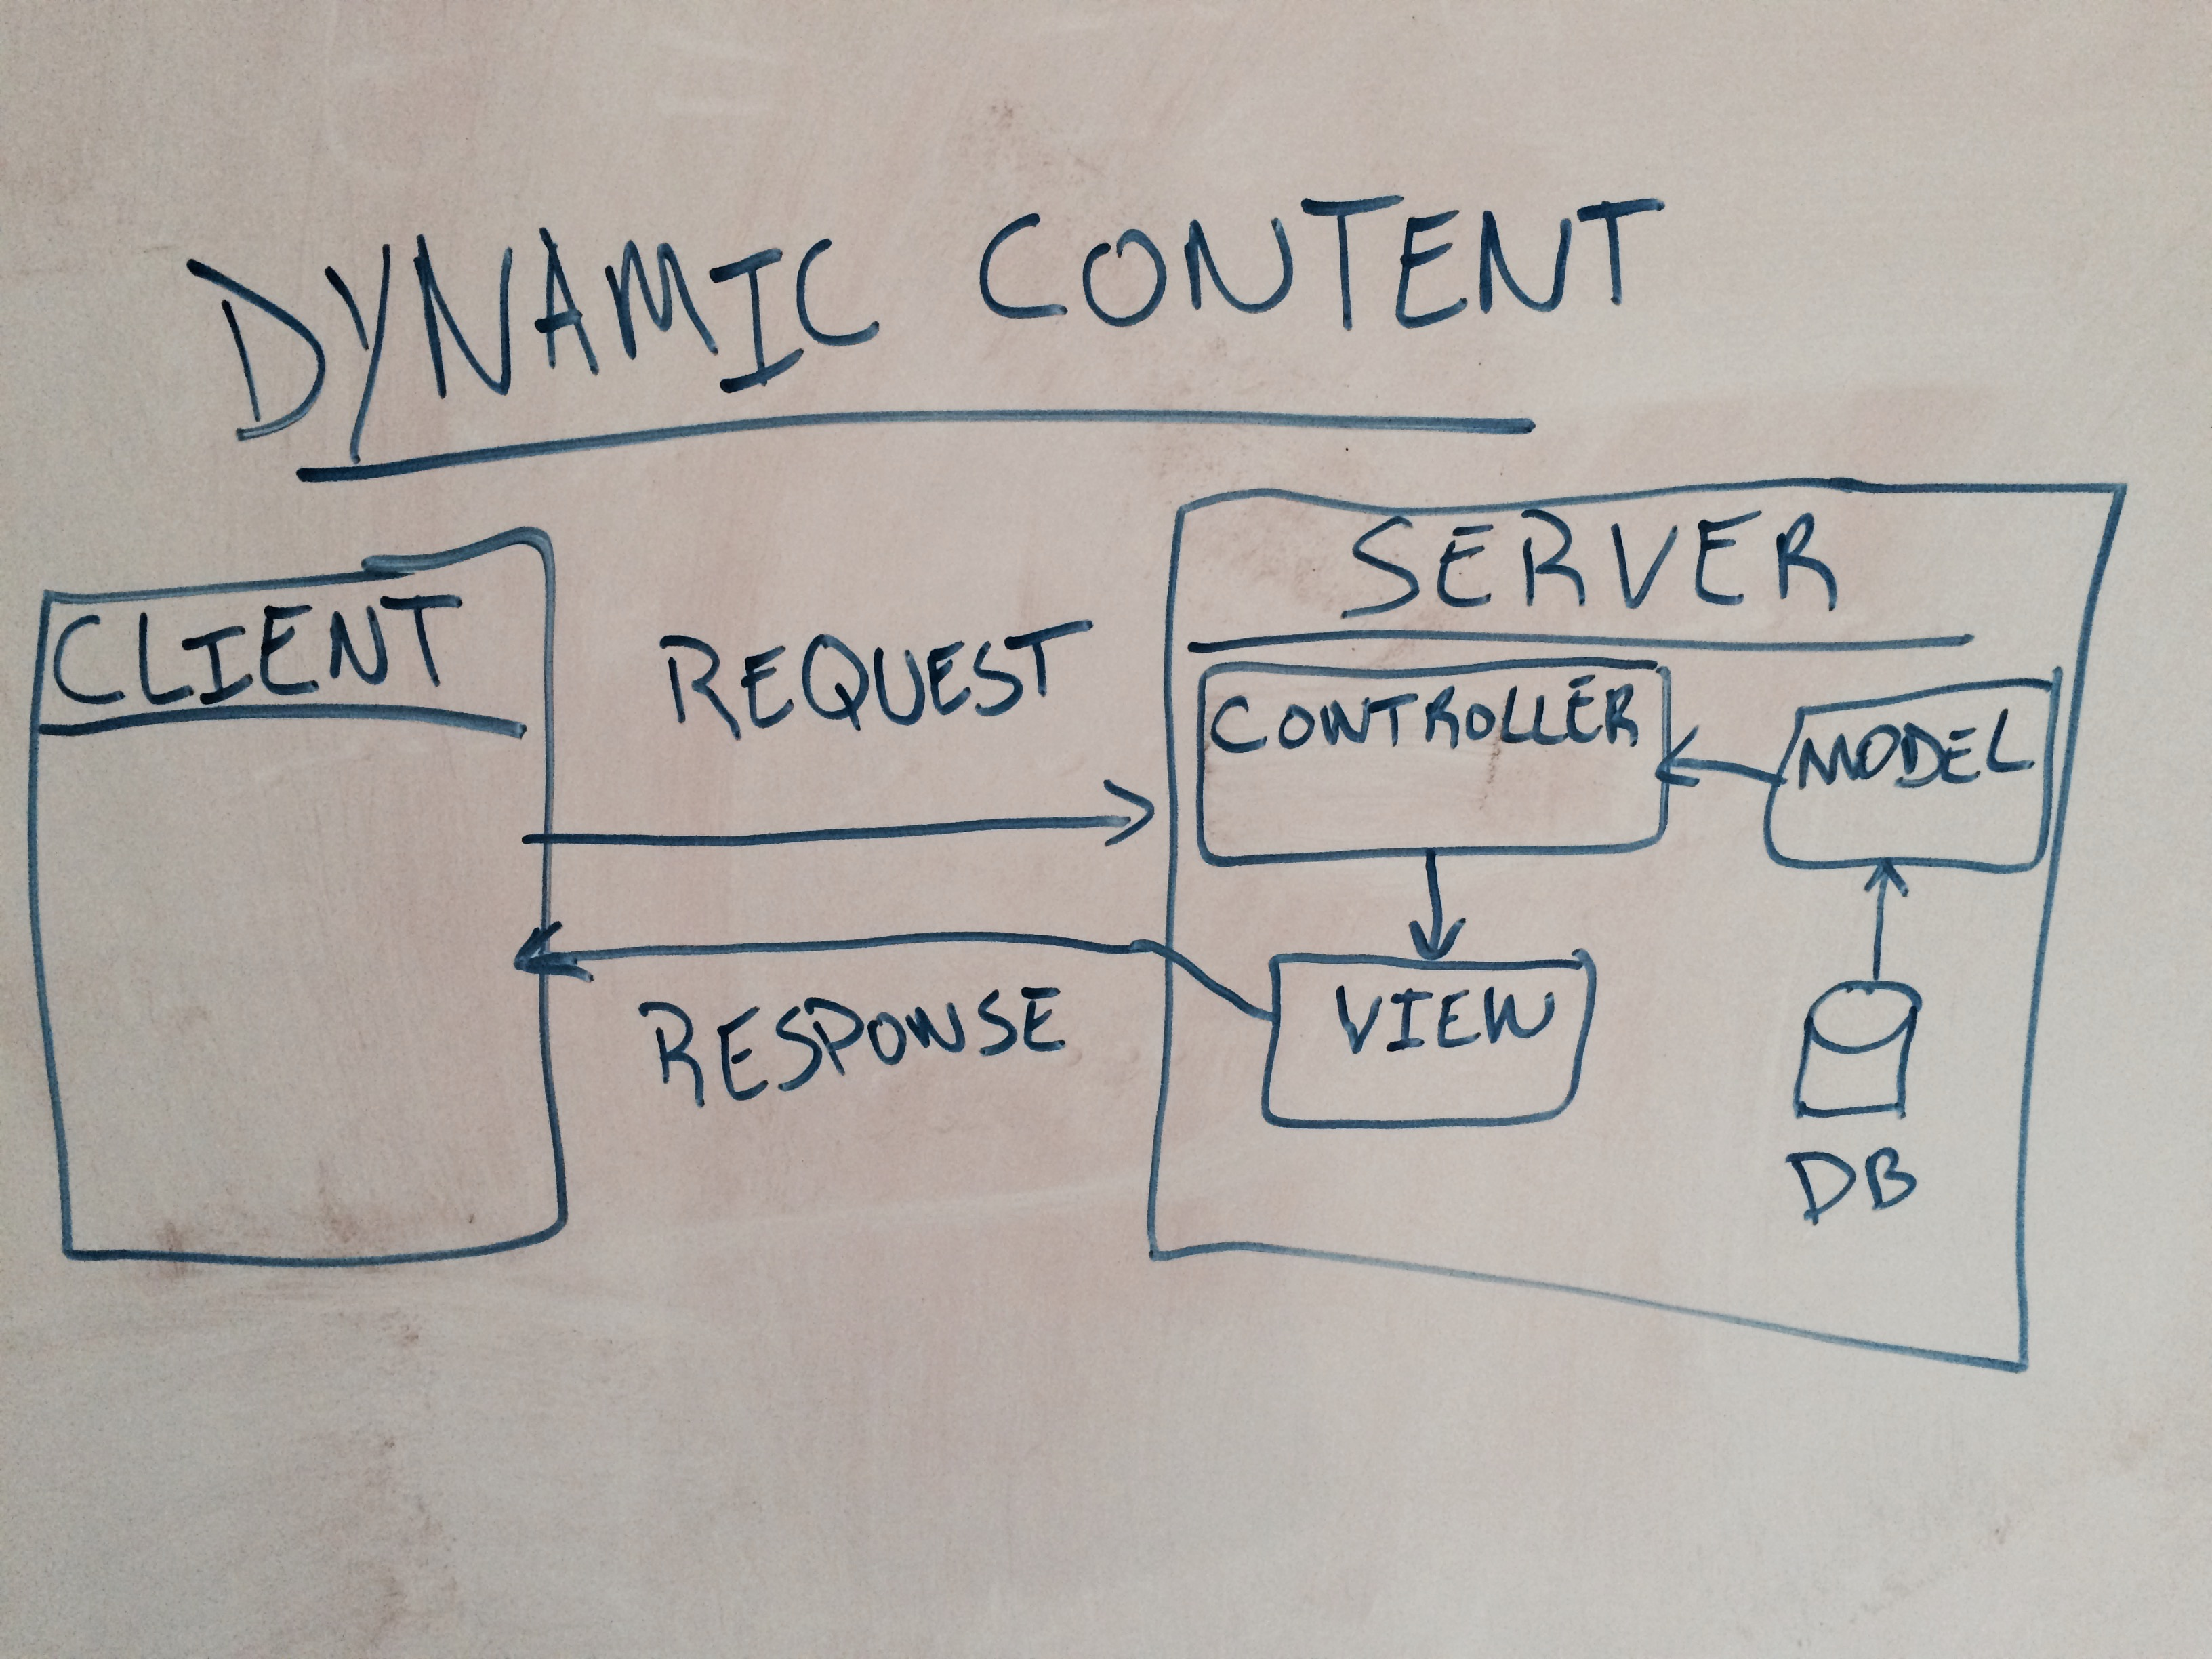
\includegraphics[scale=0.05]{../images/dynamic.jpg}
\caption{Dynamic Content}
\end{figure}
\end{columns}
\end{frame}
%------------------------------Slide2---------------------------------
\section{The Model-View-Controller Paradigm}
\begin{frame}
\frametitle{MVC in Django}
\pause
\centering
In Django \textbf{MVC} == \textbf{\alert{MVT}}
\begin{table}
\large
\centering
\begin{tabular}{|l|c|}\hline
\textbf{General}  &\textbf{Django}\\ \hline\hline
Model&Model\\ \hline
Controller&View\\ \hline
View&Template\\ \hline
\end{tabular}
\caption{\footnotesize MVC mapping in Django.}
\end{table}
\end{frame}
%------------------------------Slide3----------------------------------
\section{HTTP Verbs}
\begin{frame}
\frametitle{HTTP Verbs}
\pause
\begin{itemize}[<+->]
\item GET
\item POST
\item PUT
\item DELETE
\end{itemize}
\end{frame}
%------------------------------Slide4----------------------------------

\section{REST principles}
\begin{frame}[fragile]
\frametitle{Our app should be RESTful}
\pause
\alert{RE}presentational \alert{S}tate \alert{T}ransfer
\pause
\begin{itemize}[<+->]
\item a software architecture style consisting of guidelines and best practices for creating scalable web services (Wikipedia)
\end{itemize}
\pause
\begin{table}
\scriptsize
\centering
\begin{tabular}{|l|l|l|l|l|}\hline
Action  &URL&                  Verb  & What this does\\ \hline\hline
Index&  \texttt{/books}&       GET & show me all the books in the database\\ \hline
Show&   \texttt{/books/1}&     GET & show me a \textit{\alert{particular}} book in the database\\ \hline
New&    \texttt{/books/new}&   GET & start creating a new book\\ \hline
Create& \texttt{/books}&       POST & add a new book to the database\\ \hline
Edit&   \texttt{/books/1/edit}&GET & start making changes \textit{\alert{particular}} book \\ \hline
Update& \texttt{/books/1}&     PUT & save changes to a \textit{\alert{particular}} book in the database\\ \hline
Destroy&\texttt{/books/1}&     DELETE & delete a book from the database\\ \hline
\end{tabular}
\caption{\footnotesize Mapping REST actions to URLS and verbs.}
\end{table}
\end{frame}
%--------------------------------------------Slide5------------------------------------------------------------------
\section{Implementing RESTful principles in Django}
\begin{frame}[fragile]
\frametitle{Making our library RESTful}
\pause
\begin{table}
\scriptsize
\centering
\begin{tabular}{|l|l|l|l|l|}\hline
\textbf{Action}  &\textbf{URL}&  \textbf{Verb} & \textbf{Django URL} \\ \hline\hline
Index&    \texttt{/books}&         GET &     \texttt{/books}\\
Show&     \texttt{/books/1}&       GET &     \texttt{/books/1}\\
New&      \texttt{/books/new}&     GET &     \texttt{/books/new}\\
Create&   \texttt{/books}&         POST &    \texttt{/books/create} \\
Edit&     \texttt{/books/1/edit}&  GET &     \texttt{/books/1/edit}\\
Update&   \texttt{/books/1}&       PUT &     \texttt{/books/1/update}\\
Destroy&  \texttt{/books/1}&       DELETE &  \texttt{/books/1/destroy}\\ \hline
\end{tabular}
\caption{\footnotesize Mapping REST actions to URLS and verbs.}
\end{table}

\end{frame}
%--------------------------------------------Slide6------------------------------------------------------------------
\begin{frame}[fragile]
\frametitle{Let's take a look at our app}

\end{frame}
%--------------------------------------------Slide7------------------------------------------------------------------
\begin{frame}[fragile]
\frametitle{Let's add some content}

\end{frame}
%--------------------------------------------Slide8------------------------------------------------------------------
\begin{frame}[fragile]
\frametitle{Creating the book model}

\end{frame}
%--------------------------------------------Slide9------------------------------------------------------------------
\begin{frame}[fragile]
\frametitle{Some admin}

\end{frame}
%--------------------------------------------Slide10------------------------------------------------------------------
\begin{frame}[fragile]
\frametitle{So how do we get to see our view?}
%\begin{itemize}[<+->]
%\end{itemize}
\end{frame}
%--------------------------------------------Slide11------------------------------------------------------------------
%\section{Further Reading}
%\begin{frame}
%\frametitle{Further Reading}
%% \bibliographystyle{plain}
%% \bibliography{DevelopmentPractices.bib}
%\end{frame}
\end{document}
